\documentclass[12pt]{style/ucdavisthesis}

\usepackage[letterpaper, margin = 1in]{geometry}
% need this for the \foreach command
\usepackage{tikz}
\usetikzlibrary{calc,shapes,arrows,positioning}

% useful for drafts
% line numbers:
% http://www.ctan.org/tex-archive/help/Catalogue/entries/lineno.html
%
% \usepackage{lineno}

% more flexible math support
\usepackage{amsmath}

% allow some pages to be landscape
\usepackage{lscape}

% more flexible definition of table environments
\usepackage{ctable}

%need this for \includegraphics{}
\usepackage{graphicx}

%enable the listings package specifically for including programming code
\usepackage{listings}

%Special hack to make code listings not break pages, fyi they must be short then
\usepackage{float}
\floatstyle{plain} % optionally change the style of the new float
\newfloat{Code}{H}{myc}

%use this to put figures side by side
\usepackage{subcaption}

\usepackage[utf8]{inputenc}
\usepackage[english]{babel}

\usepackage{natbib}
\renewcommand\bibname{References}
\def\newblock{\hskip .11em plus.33em minus.07em}
\bibliographystyle{abbrvnat}
\setcitestyle{authoryear, open={(},close={)}}

\usepackage{textcomp}% for '\textdegree' macro

% custom colors
\usepackage{color}
% make a color for comments
\definecolor{MyDarkBlue}{rgb}{0,0.08,0.45}

% customized captions with bold label and small, italic text
% table captions are located above tables
\usepackage[hypcap,font=singlespacing]{caption}
%\usepackage{subcaption}
% modern method for setting up captions\
\captionsetup{margin=10pt,font=small,labelfont=bf}
%
% fix so that table captions have correct spacing
\captionsetup[table]{position=top}

\renewcommand{\floatpagefraction}{0.8}	% require fuller float pages

% N.B.: floatpagefraction MUST be less than topfraction !!
\renewcommand{\topfraction}{0.9}	% max fraction of floats at top
\renewcommand{\bottomfraction}{0.8}	% max fraction of floats at bottom

% PDF formatting options, indexing, hyperlinking, with control over link style
%Set PDF Metadata
\title{My Thesis is Too Long and Says Too Little}
\author{HRVIP Forever}
\makeatletter
\usepackage[pdftex,
            pdfauthor={\@author},
            pdftitle={\@title},
            %pdfsubject={Subject},
            %pdfkeywords={Comma, List, Keywords},
            %pdfproducer={Latex with hyperref, or other system},
            %pdfcreator={pdflatex, or other tool}
            ]{hyperref}
\makeatother
\hypersetup{
	%driver=pdftex,
	colorlinks=true,
	urlcolor=blue,
	linkcolor=blue,          % color of internal links
  citecolor=blue,        % color of links to bibliography
  filecolor=magenta
}

%Use an additional package to make bookmarks point to the top to tables, figures and listings
\usepackage[all]{hypcap}

%Alex's customizations
\usepackage{indentfirst} %Indents first paragraph of chapter
\usepackage{datatool} %Allows import of csv and other data-tables
\usepackage{varwidth}
\usepackage{color}
\usepackage{rotating}

\graphicspath{{./figures/}{./plots/}}

\newcommand{\tablepath}{./tables}

\makeatletter
\newcommand{\includetable}[1]{%
  \@ifundefined{tablepath}{%
    \InputIfFileExists{#1}{}{}%
  }{%
    \InputIfFileExists{\tablepath/#1}{}{\InputIfFileExists{#1}{}{}}%
  }
}
\makeatother

\usepackage{booktabs}
\usepackage{dcolumn}
\newcolumntype{.}{D{.}{.}{-1}}

\usepackage{csquotes}
\renewcommand\mkbegdispquote[2]{\leavevmode\llap{``}}
\renewcommand\mkenddispquote[2]{#1''#2}

\usepackage{mathtools}

\usepackage{enumitem}

\usepackage{multirow}

\usepackage{makecell}

\usepackage{nameref}

\usepackage{siunitx}
\DeclareSIUnit\inch{in}
\DeclareSIUnit\feet{ft}
\DeclareSIUnit\foot{ft}
\DeclareSIUnit\bps{bps}
\DeclareSIUnit\bits{bits}

\hyphenation{NASA-TLX}

%\usepackage[maxfloats=58]{morefloats}

\renewcommand\bibname{References}

\usepackage{flexisym}

\newcolumntype{C}[1]{>{\centering\let\newline\\\arraybackslash\hspace{0pt}}m{#1}}

\newcommand{\PreserveBackslash}[1]{\let\temp=\\#1\let\\=\temp}
\newcolumntype{R}[1]{>{\PreserveBackslash\raggedleft}p{#1}}
\newcolumntype{L}[1]{>{\PreserveBackslash\raggedright}p{#1}}

\usepackage{pifont}
\usepackage{newunicodechar}
\newunicodechar{✓}{\ding{51}}
\newunicodechar{✗}{\ding{55}}

\usepackage{adjustbox}
\usepackage[framemethod=tikz]{mdframed}

%%% Document Portion:
% Declarations for Front Matter
\title{My Thesis is Too Long and Says Too Little}
\author{HRVIP Forever}

% Choices are September, December, March, June
\degreemonth{June}
\degreeyear{3030}

\committee{Stephen K. Robinson}{Bob Clampett}{Aspiring Y. Professor}{}{}

%Your Graduate Group
\officialmajor{Mechanical and Aerospace Engineering}
\graduateprogram{Mechanical and Aerospace Engineering}

%%%%%%%%%%%%%%%%%%%%%%%%%%%%%%%%%%%%%%%%%%%%%%%%%%%%%%%%%%%%%%%%%%%%%%%%
\abstract{
  What is an abstract? What does it mean to be abstract?
}

\acknowledgments{
  Thank you to water.
  Water is important.
}

\begin{document}

% Title, Front Matter, and Abstract:
\makeintropages %Processes/produces the preliminary pages

% the chapters
\chapter{Introduction}

\section{Motivation}
I would like to have an advanced degree.

\section{Background}
I should have read the background literature before doing my research, but oh well.
I think rockets are cool.
Here's a rocket (Figure~\ref{figure:bigolrocket})!

\begin{figure}[tb]
    \begin{center}
        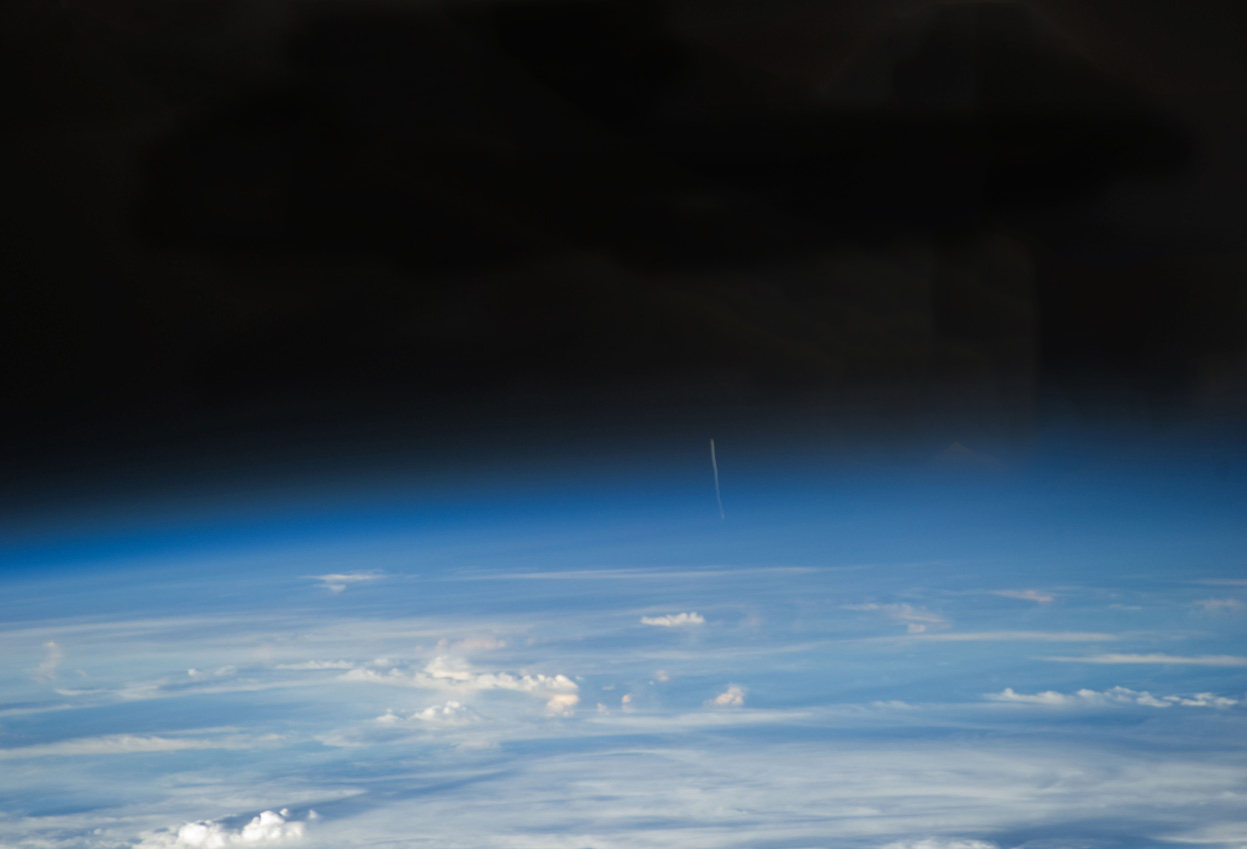
\includegraphics[width=0.33\linewidth]{figures/Introduction/ArianeLaunchFromISS.jpg}
        \caption[Rocket go vroom]{A rocket attempting to escape from Earth}
        \label{figure:bigolrocket}
    \end{center}
\end{figure}

\section{Research Questions}
It is important to have clearly defined research questions, otherwise you won't have anything to explicitly ignore:
\begin{enumerate}
    \item What is my purpose?
    \item What is the fastest path to a degree?
\end{enumerate}

\section{Summary}
I will write the greatest dissertation ever.

\chapter{Trade Study}
There are many important thing to consider when conducting a trade study.
What sorts of things \textit{are there} to study?
Which one sounds the most interesting?
Do any of them have funding?

See Table~\ref{table:first}, which is not related to this trade study.

\begin{table}[b]
    \centering
    \includetable{intro-fancy-table.tex}
    \caption[Tables are important]{Have you hugged a table today?}
    \label{table:first}
\end{table}

\chapter{Modeling}
Steve is a good model~\citep{stevewiki}.
He has a fancy suit, see Figure~\ref{figure:fancysuit}.
He wrote a good paper~\citep{robinson1991coherent}.

\begin{figure}[tb]
    \begin{center}
        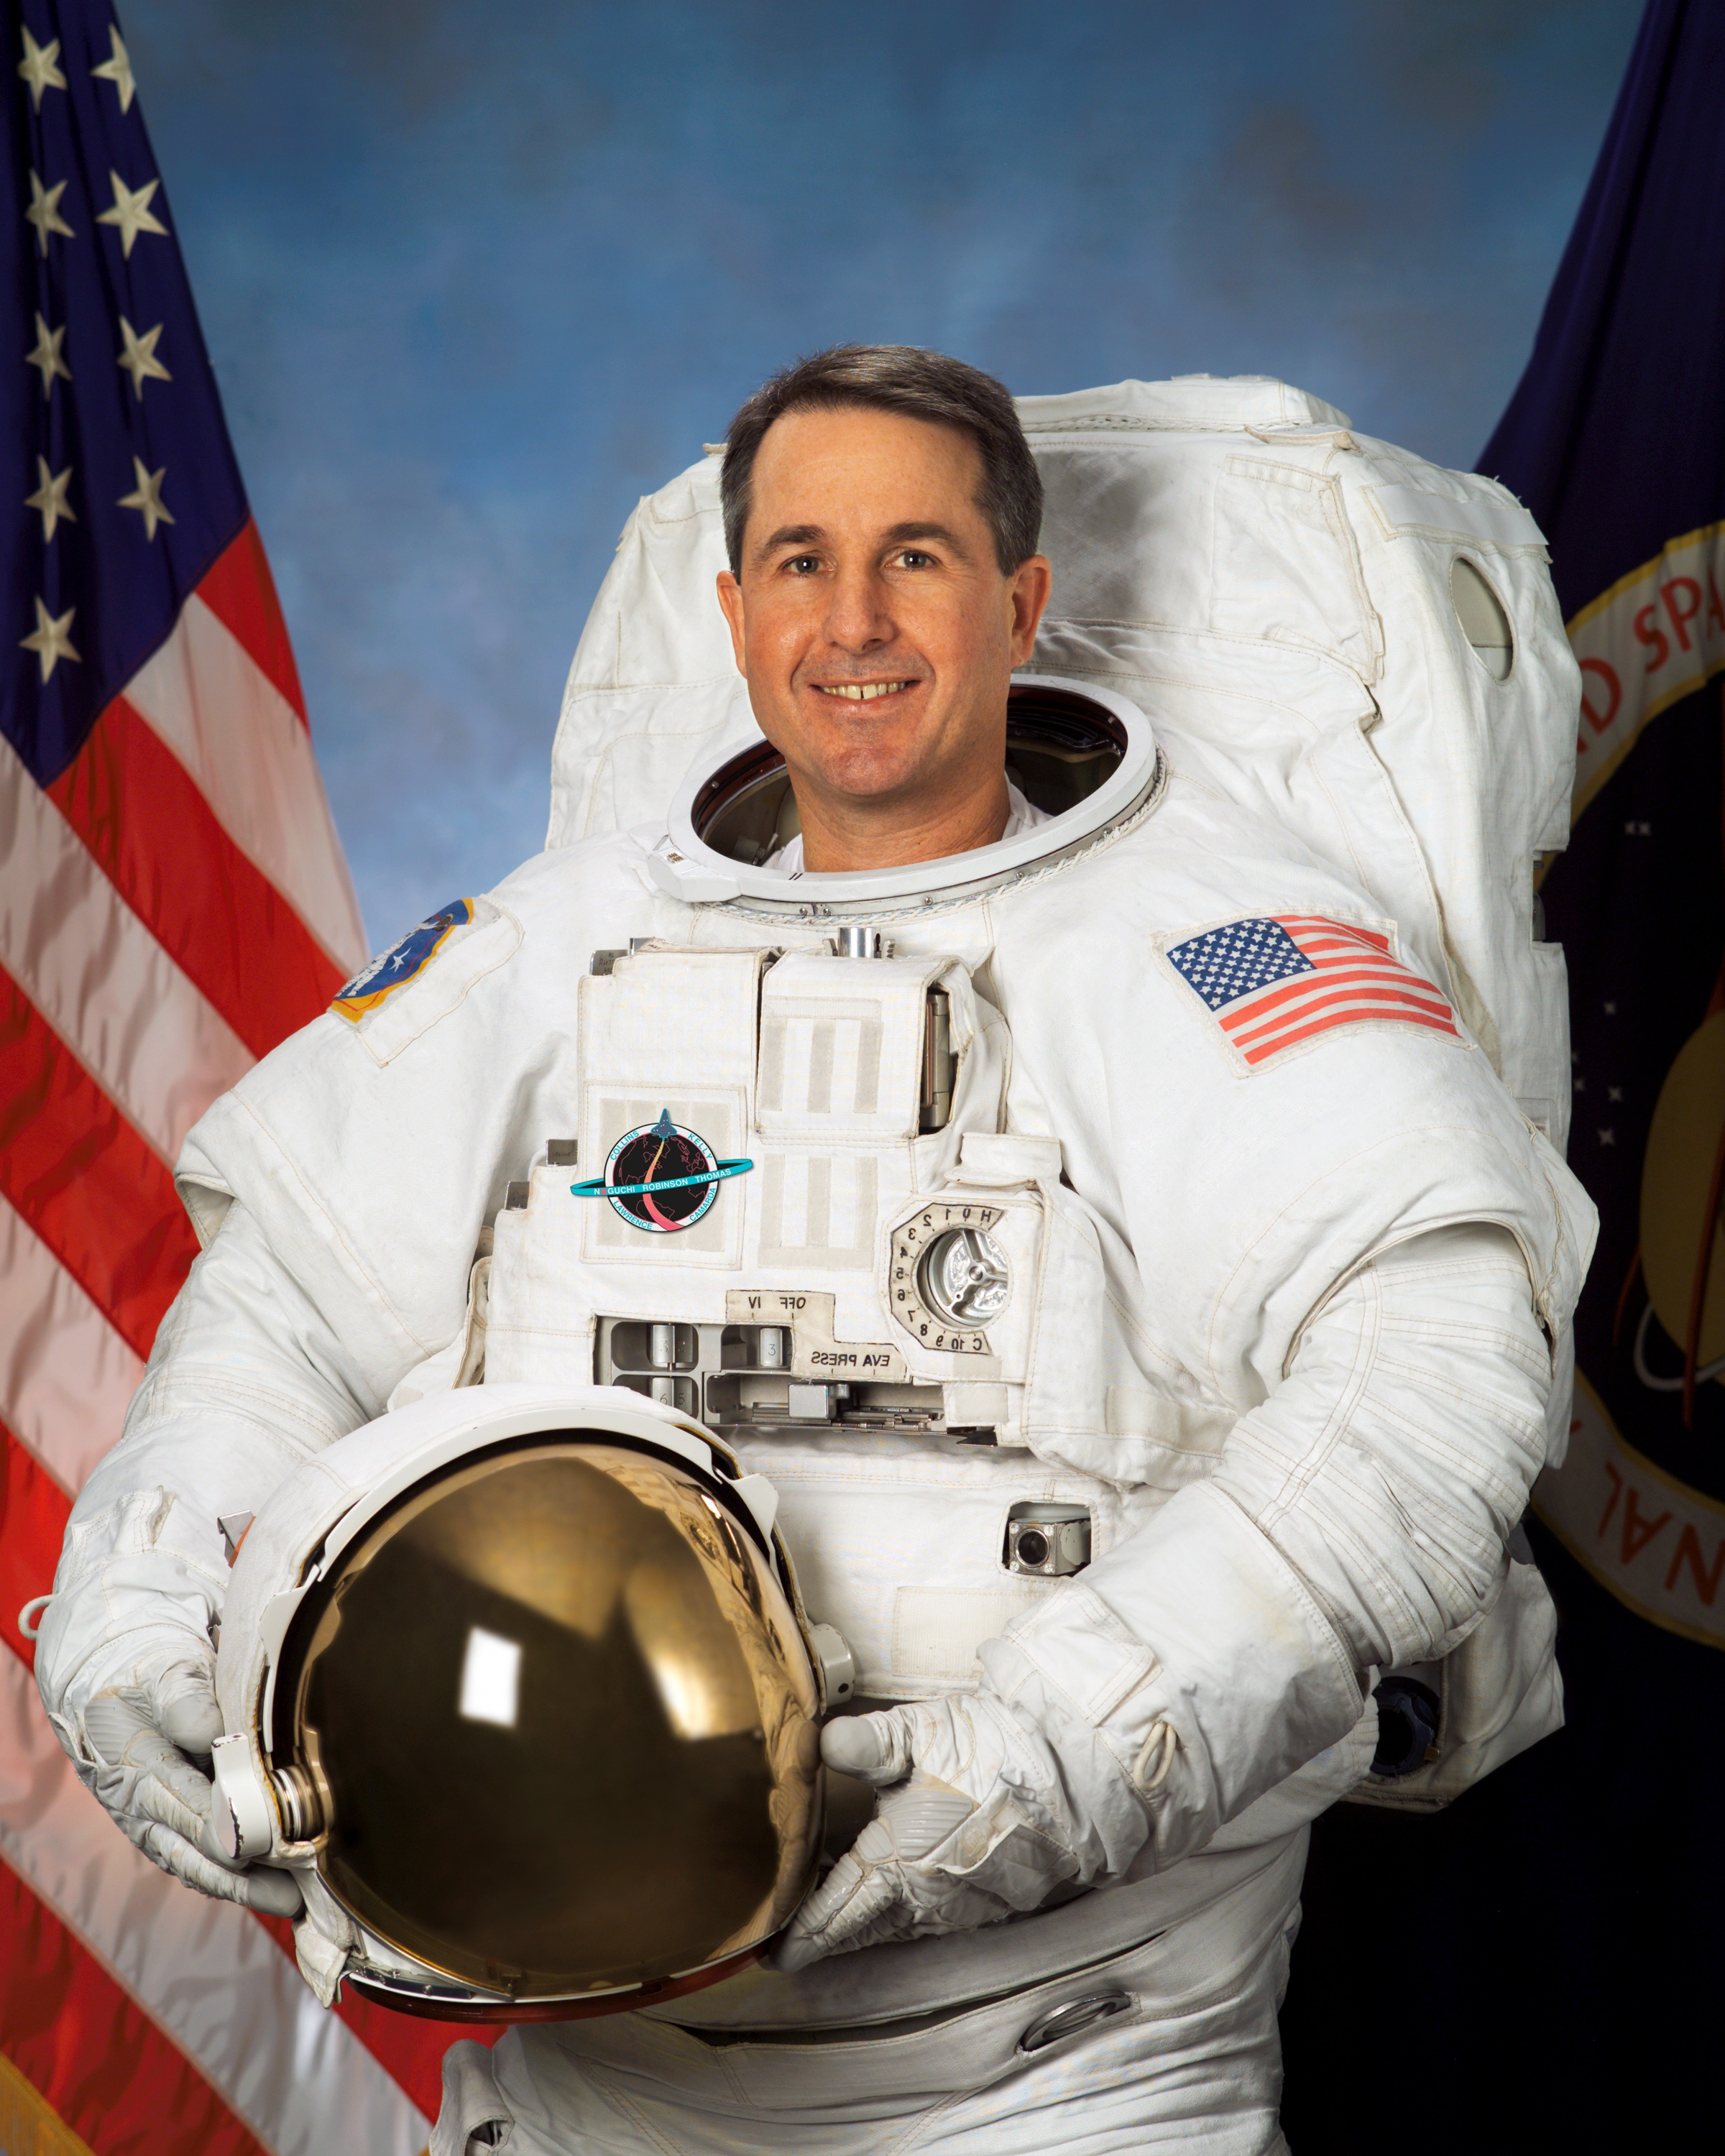
\includegraphics[width=0.25\linewidth]{figures/Modeling/Stephen_Robinson_NASA_STS114.jpg}
        \caption[Fancy suit man]{Astronaut Stephen K. Robinson, mission specialist}
        \label{figure:fancysuit}
    \end{center}
\end{figure}

\section{Introduction}
Stephen Kern Robinson (born October 26, 1955, in Sacramento, California) is a former NASA astronaut.

\section{Method}
He was active in the Boy Scouts of America where he achieved its second highest rank, Life Scout.
Robinson graduated from Campolindo High School, Moraga, California, in 1973, and obtained a Bachelor of Science degree in Mechanical and Aeronautical Engineering from the University of California, Davis in 1978, a Master of Science degree in Mechanical Engineering from Stanford University in 1985; and a Doctorate in Mechanical Engineering, with a minor in Aeronautics and Astronautics from Stanford University in 1990.

\section{Results}
He was awarded the NASA Ames Honor Award for Scientists in 1989, the American Institute of Aeronautics and Astronautics Outstanding Technical paper Award for Applied Aerodynamics in 1992, and the NASA/Space Club G. M. Low Memorial Engineering Fellowship in 1993.

\section{Discussion}
I think we will use him as a model.

\chapter{Conclusion}
In conclusion, I think I did a good job.
I don't think I wrote the best dissertation, but I'm proud of it.


% \pagestyle{plain}

\singlespacing
\bibliography{dissertation}

% the appendix:
\part*{\addcontentsline{toc}{part}{Appendices}\Huge Appendices}
\appendix

% reset page style to fancy
%\pagestyle{fancyplain}

\chapter{Personal Note}
I guess I didn't need an appendix after all.


\end{document}
